\section{二足歩行ロボットにおける歩行制御の階層構造}

二足歩行ロボットの歩行制御は，一般に複数の階層から構成される．典型的には，上位層で歩行の大局的な計画を行い，中位層で安定化を図り，下位層でロボットの全身運動を実現する構成が採られる．制御フローの全体像を \cref{fig:control_flow} に示す．

上位層では，歩行周期や足先の接地位置，重心（CoM）の目標軌道などを生成する歩行生成（walking pattern generation）が行われる．この層では，歩行の安定性や運動の滑らかさを考慮しつつ，将来の運動を計画することが主な役割となる．

中位層では，上位層で生成された参照軌道に基づき，外乱やモデル誤差に対してロボットの姿勢や運動を安定化させる安定化制御（stabilization）が行われる．この層では，重心運動や床反力を調整することで，転倒を防ぎながら歩行を継続することが求められる．
代表的な手法として，モデル予測制御（Model Predictive Control; MPC）に基づき ZMP や重心運動を調整する制御や，本研究で用いる Baseline Walking Controller（BWC）のように，歩行生成結果を基にリアルタイムで安定化補償を行う制御手法が挙げられる．これらの詳細については後述する．

下位層では，中位層で安定化された目標運動を実現するため，全身運動制御が行われる．具体的には，重心位置や足先位置などの目標を満たすように，全身逆運動学（Inverse Kinematics; IK）を解くことで各関節角度を算出し，さらに関節トルクや速度指令へと変換してアクチュエータに入力する．

本研究は，これらの階層のうち，特に歩行生成および安定化制御における重心運動の扱いに着目する．関節制御や逆運動学の詳細な実装については既存手法を用いるものとし，本論文では扱わない．

\begin{figure}[htbp]
  \centering
  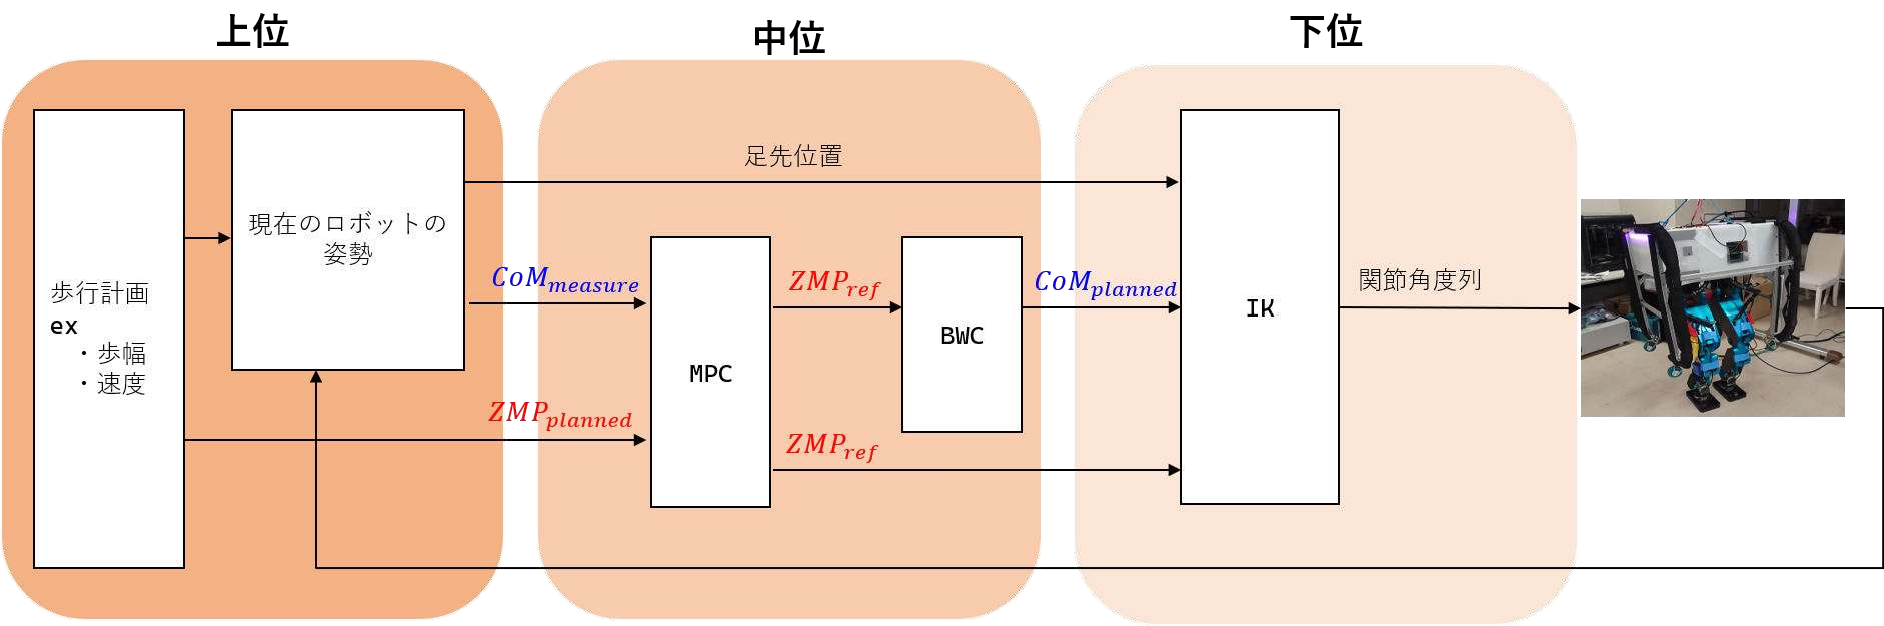
\includegraphics[width=1.0\linewidth]{images/control_flow.pdf}
  \caption{二足歩行ロボットの制御フロー}
  \label{fig:control_flow}
\end{figure}
